\documentclass{article}
\usepackage[utf8]{inputenc}
\usepackage{tikz}
\usetikzlibrary{positioning}
\usetikzlibrary{shapes.geometric, arrows}
\begin{document}




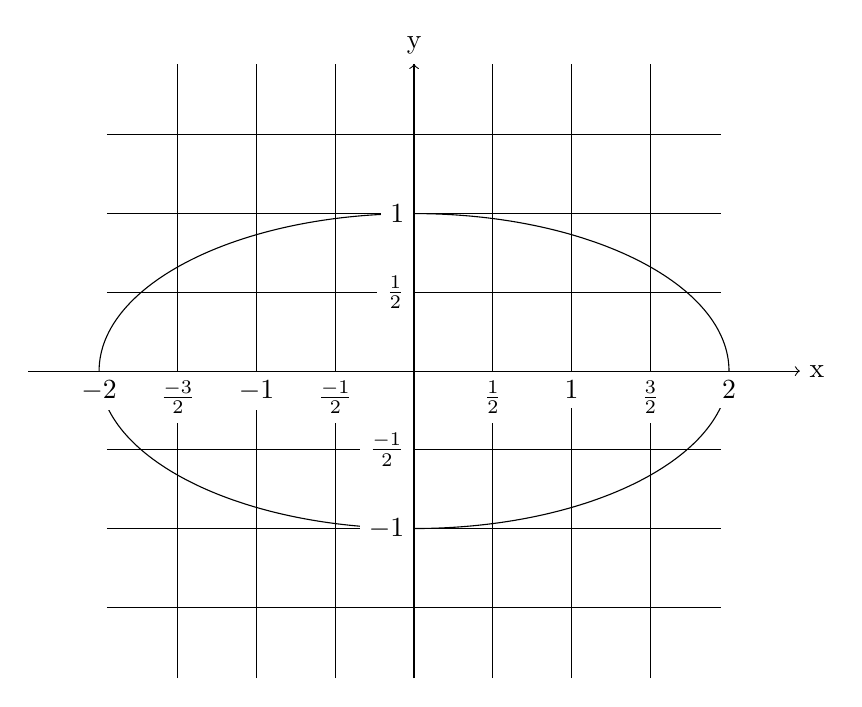
\begin{tikzpicture}
    \draw (-3.9,-3.9) grid (3.9,3.9);
    \draw[->] (-4.9,0) -- (4.9,0) node[right] {x};
    \draw[->] (0,-3.9) -- (0,3.9) node[above] {y};
     \draw (0,0) ellipse (4cm and 2cm);


    \tikzstyle{every node} = [fill=white];
    \node at (-1,0) [below] {$-1\over2$};
    \node at (-2,0) [below] {$-1$};
     \node at (-3,0) [below] {$-3\over2$};
    \node at (-4,0) [below] {$-2$};
    \node at (1,0) [below] {$1\over2$};
    \node at (2,0) [below] {$1$};
     \node at (3,0) [below] {$3\over2$};
    \node at (4,0) [below] {$2$};
    \node at (0,-1) [left] {$-1\over2$};
    \node at (0,-2) [left] {$-1$};
    \node at (0,1) [left] {$1\over2$};
    \node at (0,2) [left] {$1$};
\end{tikzpicture}







\\\\

\tikzstyle{roundnode}=[circle,draw=green!60,fill=green!5,very thick, minimum size=7mm]
\tikzstyle{squarednode}=[rectangle,draw=red!60,fill=red!5,very thick, minimum size=5mm]



\begin{tikzpicture}
    % \draw[blue] (-2,-2) grid (6,6);
    \node[roundnode] (1) {X};
    \node[squarednode] (2) [right=of 1] {f(x)};
    \node[squarednode] (3) [right=of 2] {g(x)};
    \node[squarednode] (4) [below=of 3] {h(x)};
    \draw[->] (-2,0) -- (1.west);
    \draw[->] (3.east) -- (6,0);
    \draw[->] (1.east) -- (2.west);
    \draw[->] (2.east) -- (3.west);
    \draw[->] (5,0) to [out=290, in=0] (4.east);
    \draw (4.west) -- (0,-1.6);
    \draw[->] (0,-1.6) -- (1.south);
    
    \node at (-1,0) [text=black, above] {$y_0$};
    \node at (0.7,0) [text=black, above] {$ \sigma  $};
    \node at (5,0) [text=black, above] {$y$};
    \node at (0,-1) [text=black, left] {$y_w$};
    \node at (2.7,0) [text=black, above] {$\mu$};
\end{tikzpicture}


\end{document}